\documentclass[nobib]{tufte-handout}

%\\geometry{showframe}% for debugging purposes -- displays the margins

\newcommand{\bra}[1]{\left(#1\right)}
\usepackage{amssymb}
\usepackage{hyperref}
\usepackage{pgfplots}
\usepackage[activate={true,nocompatibility},final,tracking=true,kerning=true,spacing=true,factor=1100,stretch=10,shrink=10]{microtype}
\usepackage{color}
\usepackage{steinmetz}
\usepackage{placeins}
% Fixes captions and images being cut off
\usepackage{marginfix}
\usepackage{array}
\usepackage{tikz}
\usepackage{amsmath,amsthm}
\usetikzlibrary{shapes, arrows, positioning, calc}
\tikzset{block/.style={draw, rectangle, minimum height=1.5em, minimum width=3em},
         sum/.style={draw, circle, inner sep=0pt, minimum size=2mm},
         >=latex'}
\usepackage{listings}
\usepackage{forest}
\usepackage{caption}
\DeclareCaptionFont{white}{\color{white}}
\DeclareCaptionFormat{listing}{\colorbox{gray}{\parbox{\textwidth}{#1#2#3}}}
\captionsetup[lstlisting]{format=listing,labelfont=white,textfont=white}

% Set up the images/graphics package
\usepackage{graphicx}
\setkeys{Gin}{width=\linewidth,totalheight=\textheight,keepaspectratio}
\graphicspath{{.}}

\title{Notes for ECE 30100 - Signals and Systems}
\author{Zeke Ulrich}
\date{\today}  % if the \date{} command is left out, the current date will be used

% The following package makes prettier tables.  We're all about the bling!
\usepackage{booktabs}

% The units package provides nice, non-stacked fractions and better spacing
% for units.
\usepackage{units}

% The fancyvrb package lets us customize the formatting of verbatim
% environments.  We use a slightly smaller font.
\usepackage{fancyvrb}
\fvset{fontsize=\normalsize}

% Small sections of multiple columns
\usepackage{multicol}

% For finite state machines 
\usetikzlibrary{automata} % Import library for drawing automata
\usetikzlibrary{positioning} % ...positioning nodes
\usetikzlibrary{arrows} % ...customizing arrows
\tikzset{node distance=2.5cm, % Minimum distance between two nodes. Change if necessary.
    every state/.style={ % Sets the properties for each state
    semithick,
    fill=gray!10},
    initial text={}, % No label on start arrow
    double distance=2pt, % Adjust appearance of accept states
    every edge/.style={ % Sets the properties for each transition
    draw,
    ->,>=stealth', % Makes edges directed with bold arrowheads
    auto,
    semithick}}
\let\epsilon\varepsilon

% These commands are used to pretty-print LaTeX commands
\newcommand{\doccmd}[1]{\texttt{\textbackslash#1}}% command name -- adds backslash automatically
\newcommand{\docopt}[1]{\ensuremath{\langle}\textrm{\textit{#1}}\ensuremath{\rangle}}% optional command argument
\newcommand{\docarg}[1]{\textrm{\textit{#1}}}% (required) command argument
\newenvironment{docspec}{\begin{quote}\noindent}{\end{quote}}% command specification environment
\newcommand{\docenv}[1]{\textsf{#1}}% environment name
\newcommand{\docpkg}[1]{\texttt{#1}}% package name
\newcommand{\doccls}[1]{\texttt{#1}}% document class name
\newcommand{\docclsopt}[1]{\texttt{#1}}% document class option name

% Define a custom command for definitions and biconditional
\newcommand{\defn}[2]{\noindent\textbf{#1}:\ #2}
\let\biconditional\leftrightarrow

\begin{document}

\maketitle

\tableofcontents

\section{Course Description}
Classification, analysis and design of systems in both the time- and frequency-domains.
Continuous-time linear systems: Fourier Series, Fourier Transform, bilateral Laplace
Transform. Discrete-time linear systems: difference equations, Discrete-Time Fourier
Transform, bilateral z-Transform. Sampling, quantization, and discrete-time processing
of continuous-time signals. Discrete-time nonlinear systems: median-type filters,
threshold decomposition. System design examples such as the compact disc player and AM radio.
\pagebreak

\section{Introduction}
Let's examine some basic C++ programs.
\begin{lstlisting}[language=C++,caption=Hello World]
    #include <iostream>

    int main() {
        std::cout << "Hello World!";
        return 0;
    }
\end{lstlisting}

\begin{lstlisting}[language=C++,caption=User Input]
    #include <iostream>

    int main() {
        double n;
        int i;

        std::cout << "Enter float: ";
        std::cin >> n;

        std::cout << "Enter integer: ";
        std::cin >> i;

        return 0;
    }
\end{lstlisting}

The \texttt{stds} you're seeing all over the place refer not
to a frat party but the standard namespace. It holds
useful objects like standard in ("\texttt{cin}") and standard
out ("\texttt{cout}").

In C, we use \texttt{malloc} and \texttt{free} to allocate memory. In C++,
the equivalent operations are \texttt{new} and \texttt{delete}.

\begin{lstlisting}[language=C++,caption=Free and Delete]
    void CorrectUsage(){
        int *ptr = new int[3];
        int *ptr1 = new int;
        ptr[0] = 1;
        ptr[1] = 2;
        ptr[2] = 3;
        *ptr1 = 5;
        delete ptr1;
        delete [] ptr;        
\end{lstlisting}
The reason for this is using \texttt{new} and \texttt{free} calls
an object's constructor and destructors, which are defined to properly
delete the object. Technically, \texttt{malloc} and \texttt{free} are
both present in C++, but they won't trigger the constructors and
destructors and should be avoided. The choice to leave these functions in
was made to improve compatibility with C, which is a theme the reader
may notice in C++'s many possible ways to do the same thing.

C++ filenames are terminated with a \texttt{.cpp} or \texttt{.cc}
extension, like \texttt{example.cpp} or \texttt{example.cc}
\section{Linearity}
Readers are familiar with the concept
of linearity, which mathematically
may be expressed as
\begin{equation}
    f(a + b) = f(a) + f(b)
\end{equation}

Linear systems possess the property
of superposition, so given an
input as a sum of weighted inputs
the output is a sum of weighted outputs.

The necessary and sufficient
conditions for linearity in a CT
system are
if the input is $\alpha_1x_1(t)
    + \alpha_2x_2(t)$ the output
is $S(\alpha_1x_1(t)) + S(\alpha_2x_2(t))$.
Formally,
\begin{equation}
    S(\alpha_1x_1(t) + \alpha_2x_2(t)) = \alpha_1S(x_1(t)) + \alpha_2S(x_2(t)).
\end{equation}
Likewise for DT systems,
\begin{equation}
    S[\alpha_1x_1[t] + \alpha_2x_2[t]] = \alpha_1S[x_1[t]] + \alpha_2S[x_2[t]].
\end{equation}
This equality for hold for any real
valued $\alpha_1$ and $\alpha_2$.

Consider the CT system $S$ given
by $y(t) = tx(t)$. We are interested
in determining if the system is
linear. We test it with the definition
of linearity,
\begin{align}
    y(\alpha_1x_1(t) + \alpha_2x_2(t)) & = t(\alpha_1x_1(t) + \alpha_2x_2(t))    \\
                                       & = t\alpha_1x_1(t) + t\alpha_2x_2(t)     \\
                                       & = \alpha_1y(x_1(t)) + \alpha_2y(x_2(t))
\end{align}
Since this is the definition of linearity, the
system is linear.

Why do we care? We care because linearity
gives us many useful properties and
makes solving systems much easier.
If we know the output for any set of
inputs, we can find the output for
any linear combination of those inputs.

\section{Classifying Signal Types}
Before we proceed we must be able to classify signal types.
There are five ways to divide signal types.
\begin{itemize}
    \item DT vs. CT
    \item Periodic vs. aperiodic
    \item Finite energy vs. finite power
    \item Even and odd
    \item Complex exponential
\end{itemize}

\subsection{DT vs. CT}
\begin{itemize}
    \item DT: $x[n]$ is a sequence of complex values, including purely real values.
          numbers. Example: $x[n] = \frac{n}{2}$.
    \item CT: $x(t)$ is complex (including purely real) and continuous for all real values of $t$.
          Example: $x(t) = \frac{t}{2} -jt$.
    \item Complex:
\end{itemize}

For DT, complex $x[n]$ can be represented in Cartesian or polar form.
For Cartesian,
\begin{equation}
    x[n] = x_{Re}[n] + jx_{Im}[n].
\end{equation}
For polar,
\begin{equation}
    x[n] = A[n]e^{j\Theta[n]}.
\end{equation}
We can swap between the two with Euler's formula.
\begin{align}
    A[n]e^{j\Theta[n]}     & = A[n]\cos(\Theta[n]) + jA[n]\sin(\Theta[n])                                        \\
    x_{Re}[n] + jx_{Im}[n] & = \sqrt{x_{Re}[n]^2 + x_{Im}[n]^2} \times e^{j\arctan(\frac{x_{Im}[n]}{x_{Re}[n]})}
\end{align}

\subsection{Energy vs. Power}
DT vs. CT is one option to classify signals. Another
possibility is Energy vs. Power. For this class, energy in a continuous
time system is the area under the squared magnitude of the signal. Mathematically
energy over $(t_1, t_2)$ is equal to
\begin{align}
    E & = \int_{t_1}^{t_2} |x(t)|^2 dt                     \\
      & = \int_{t_1}^{t_2} (x_{Re}(t)^2 + x_{Im}(t)^2) dt.
\end{align}
For DT systems, the formula for energy is
\begin{align}
    E & = \sum_{n=n_1}^{n_2} |x[n]|^2                     \\
      & = \sum_{n=n_1}^{n_2} (x_{Re}[n]^2 + x_{Im}[n]^2).
\end{align}
The total energy $E_\infty$ is the energy from $t = -\infty$ to $t = \infty$.

Power is energy per unit time, or in terms of calculus $P(t) = \frac{d}{dt}E(t)$.
For CT, average power is
\begin{equation}
    P_{avg} = \frac{1}{t_2 - t_1} \int_{t_1}^{t_2} |x(t)|^2 dt.
\end{equation}
For DT,
\begin{equation}
    P_{avg} = \frac{1}{n_2 - n_1 + 1} \sum_{n=n_1}^{n_2} |x[n]|^2.
\end{equation}
The overall average power is
\begin{equation}
    P_{\infty} = \lim_{T \rightarrow \infty} \frac{1}{2T} \int_{-T}^{T} |x(t)|^2 dt
\end{equation}
for CT and
\begin{equation}
    P_{\infty} = \lim_{N \rightarrow \infty} \frac{1}{2N + 1} \sum_{n=-N}^{N} |x[n]|^2
\end{equation}
for DT time.
\section{Transformations}
Just as with functions, signals can be transformed in time. Here are the different transformations that can be applied to signals.

\subsection{Time Shift}
A CT time shift is given by $x(t) \rightarrow x(t-t_0)$, where $t_0$ is real.
\begin{itemize}
    \item $t_0 > 0$: shifted to the right or delayed by $t_0$
    \item $t_0 < 0$: shifted to the left or advanced by $t_0$
\end{itemize}
A DT time shift is given by $x[n] \rightarrow x[n - n_0]$, where $n_0$ is an integer.
\begin{itemize}
    \item $n_0 > 0$: shifted to the right or delayed by $n_0$
    \item $n_0 < 0$: shifted to the left or advanced by $n_0$
\end{itemize}

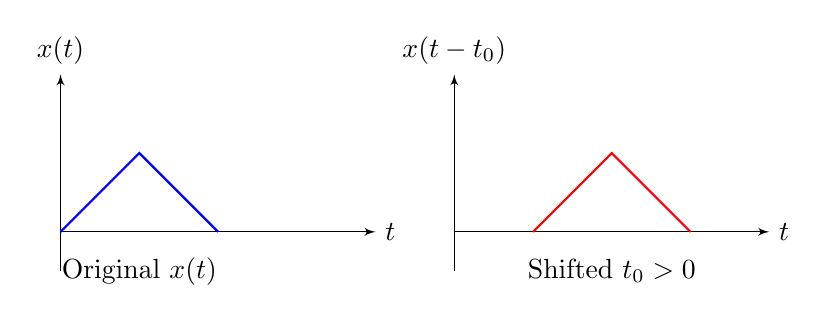
\begin{tikzpicture}
    % Original signal
    \draw[->] (0, 0) -- (4, 0) node[right] {$t$};
    \draw[->] (0, -0.5) -- (0, 2) node[above] {$x(t)$};
    \draw[thick, blue] (0, 0) -- (1, 1) -- (2, 0);
    \node at (1, -0.5) {Original $x(t)$};

    % Shifted signal
    \begin{scope}[shift={(5, 0)}]
        \draw[->] (0, 0) -- (4, 0) node[right] {$t$};
        \draw[->] (0, -0.5) -- (0, 2) node[above] {$x(t - t_0)$};
        \draw[thick, red] (1, 0) -- (2, 1) -- (3, 0);
        \node at (2, -0.5) {Shifted $t_0 > 0$};
    \end{scope}
\end{tikzpicture}

\subsection{Time Reversal}
A CT time reversal is given by $x(t) \rightarrow x(-t)$. A DT time reversal is given by $x[n] \rightarrow x[-n]$.

\begin{tikzpicture}
    % Original signal
    \draw[->] (-4, 0) -- (2, 0) node[right] {$t$};
    \draw[->] (0, -0.5) -- (0, 2) node[above] {$x(t)$};
    \draw[thick, blue] (-2, 0) -- (-1, 1) -- (0, 0);
    \node at (-1.5, -0.5) {Original $x(t)$};

    % Reversed signal
    \begin{scope}[shift={(5, 0)}]
        \draw[->] (-2, 0) -- (4, 0) node[right] {$t$};
        \draw[->] (0, -0.5) -- (0, 2) node[above] {$x(-t)$};
        \draw[thick, red] (0, 0) -- (1, 1) -- (2, 0);
        \node at (1.5, -0.5) {Reversed};
    \end{scope}
\end{tikzpicture}

\subsection{Time Scaling}
A CT time scaling is given by $x(t) \rightarrow x(\alpha t)$, where $\alpha > 0$ is the time scaling factor.
\marginnote{If $\alpha < 0$, that's viewed as a combination of reversal and scaling.}
\begin{itemize}
    \item $\alpha > 1$: shorter timescale, or sped up
    \item $\alpha < 1$: longer timescale, or slowed down
\end{itemize}
A DT time scaling is given by $x[n] \rightarrow x[\alpha n]$.

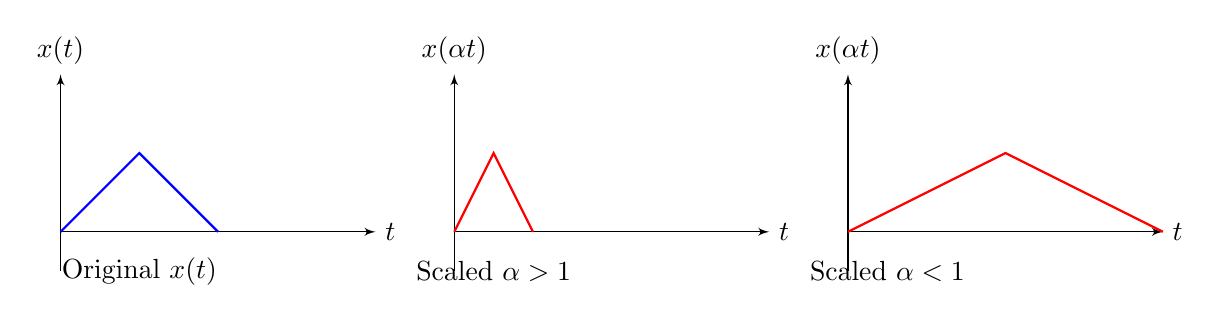
\begin{tikzpicture}
    % Original signal
    \draw[->] (0, 0) -- (4, 0) node[right] {$t$};
    \draw[->] (0, -0.5) -- (0, 2) node[above] {$x(t)$};
    \draw[thick, blue] (0, 0) -- (1, 1) -- (2, 0);
    \node at (1, -0.5) {Original $x(t)$};

    % Scaled signal
    \begin{scope}[shift={(5, 0)}]
        \draw[->] (0, 0) -- (4, 0) node[right] {$t$};
        \draw[->] (0, -0.5) -- (0, 2) node[above] {$x(\alpha t)$};
        \draw[thick, red] (0, 0) -- (0.5, 1) -- (1, 0);
        \node at (0.5, -0.5) {Scaled $\alpha > 1$};
    \end{scope}

    \begin{scope}[shift={(10, 0)}]
        \draw[->] (0, 0) -- (4, 0) node[right] {$t$};
        \draw[->] (0, -0.5) -- (0, 2) node[above] {$x(\alpha t)$};
        \draw[thick, red] (0, 0) -- (2, 1) -- (4, 0);
        \node at (0.5, -0.5) {Scaled $\alpha < 1$};
    \end{scope}
\end{tikzpicture}

A signal is even if it's symmetric with respect 
to the dependent axis. Mathematically, 
if $x(t) = x(-t)$. 

A signal is odd if it's symmetric with respect to the 
origin. Mathematically, if $x(-t) = -x(t)$. 

\begin{figure}
    \centering
    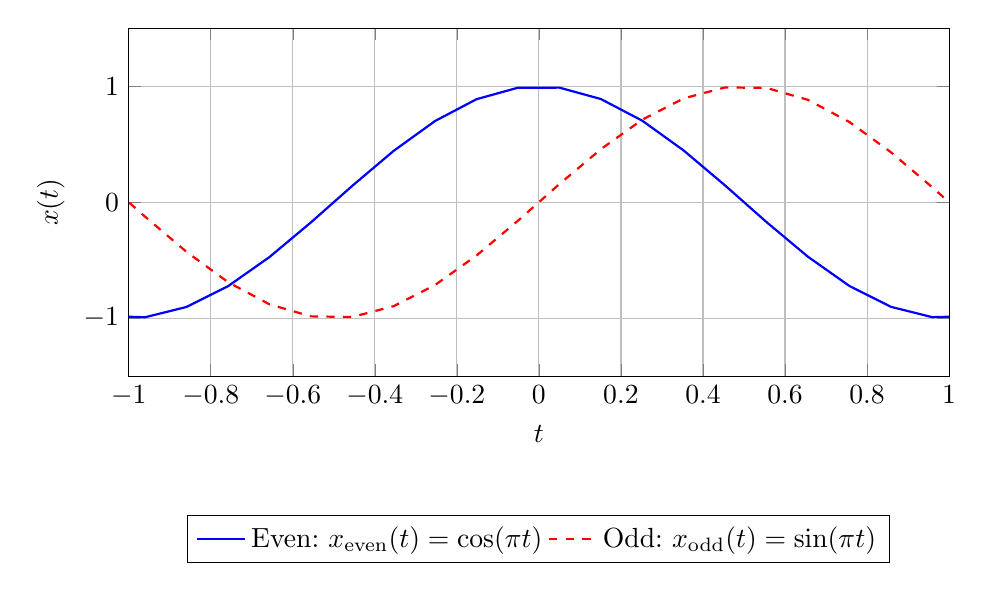
\begin{tikzpicture}
        \begin{axis}[
            width=12cm, height=6cm,
            xlabel={$t$}, ylabel={$x(t)$},
            grid=both,
            legend style={at={(0.5,-0.4)}, anchor=north, legend columns=2},
            xmin=-1, xmax=1,
            ymin=-1.5, ymax=1.5,
            samples=100
        ]
        \addplot[blue, thick] {cos(deg(pi*x))};
        \addlegendentry{Even: $x_\text{even}(t) = \cos(\pi t)$};
    
        \addplot[red, thick, dashed] {sin(deg(pi*x))};
        \addlegendentry{Odd: $x_\text{odd}(t) = \sin(\pi t)$};
        \end{axis}
    \end{tikzpicture}
    \caption{Even and odd signals}
    \end{figure}

Signals can be odd, even, both, or neither. $x(t) = 0$, 
for instance, is both even and odd. $x + 1$ is neither. 

The product of two odd signals is even (e.g. $x \times x^3$). 
The product of two evens is even ($x^2 \times 2$). The product of 
an odd and an even is odd ($x \times x^2$). 

Any signal can be written as the sum of an even and an odd signal. 
\section{Periodicity}

A system is periodic if $x(t) = x(t + T)$, or 
in the case of discrete time, if $x[n] = x[n + N]$. 


% Periodic Continuous-Time Signal
\begin{figure}
    \centering
    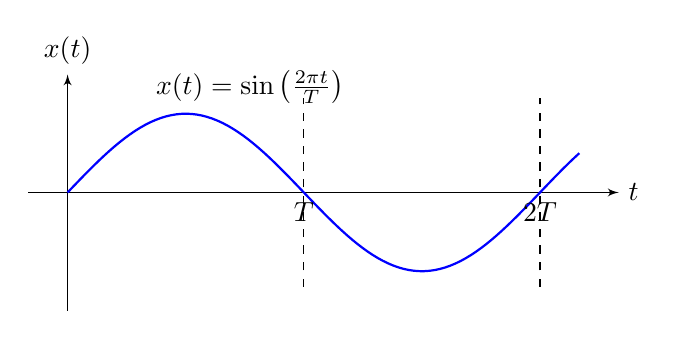
\begin{tikzpicture}[scale=1]
        % Axes
        \draw[->] (-0.5, 0) -- (7, 0) node[right] {$t$};
        \draw[->] (0, -1.5) -- (0, 1.5) node[above] {$x(t)$};
    
        \draw[thick, blue, domain=0:6.5, samples=100] plot (\x, {sin(60*\x)});
    
        % T markings
        \node[below] at (3, 0) {$T$};
        \draw[dashed] (3, -1.2) -- (3, 1.2);
        \node[below] at (6, 0) {$2T$};
        \draw[dashed] (6, -1.2) -- (6, 1.2);
    
        % Labels
        \node[above right] at (1, 1) {$x(t) = \sin\left(\frac{2\pi t}{T}\right)$};
    \end{tikzpicture}
    \caption{Periodic CT Signal}
\end{figure}
    
\begin{figure}
    \centering
    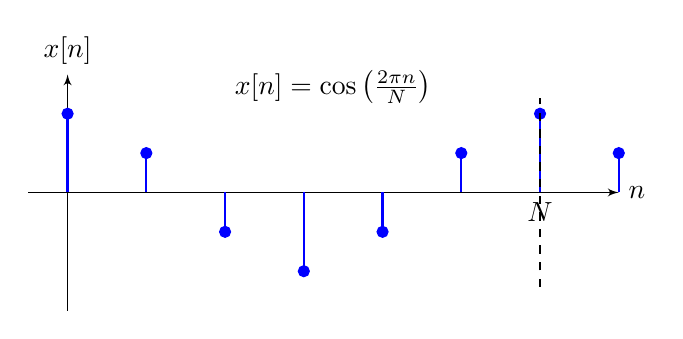
\begin{tikzpicture}[scale=1]
        % Axes
        \draw[->] (-0.5, 0) -- (7, 0) node[right] {$n$};
        \draw[->] (0, -1.5) -- (0, 1.5) node[above] {$x[n]$};
    
        % Stem plot for a cosine signal
        \foreach \n in {0, 1, ..., 7} {
            \draw[thick, blue] (\n, 0) -- (\n, {cos(60*\n)});
            \filldraw[blue] (\n, {cos(60*\n)}) circle (0.07);
        }
    
        % T markings
        \node[below] at (6, 0) {$N$};
        \draw[dashed] (6, -1.2) -- (6, 1.2);
    
        % Labels
        \node[above right] at (2, 1) {$x[n] = \cos\left(\frac{2\pi n}{N}\right)$};
    \end{tikzpicture}
    \caption{Periodic DT Signal}
\end{figure}

The fundemental period is the smallest $T_0$ (or $N_0$) such 
that $x(t) = x(t + T_0)$ (or $x[n] = x[n + N_0]$). If $x(t)$ is periodic, $x_{Re}(t) + j x_{Im}(t)$ is also 
periodic. However, if $x_1(t)$ and $x_2(t)$ are periodic then it is not 
necessarily the case that $x_1(t) + x_2(t)$ is 
periodic. Consider $x_1(t) = \sin(t)$ and 
$x_2(t) = \sin(\sqrt{2} t)$. $x_1(t) + x_2(t) = \sin(t) + \sin(\sqrt{2}t)$.
$x_1(t)$ has period $2\pi$. $x_2(t)$ has period $\frac{2\pi}{\sqrt{2}}$. 
However, their sum is not periodic and in fact the sum of 
any $x_1(t)$, $x_2(t)$ will be aperiodic when the ratio 
of their periods is irrational. 

\begin{figure}
    \centering
    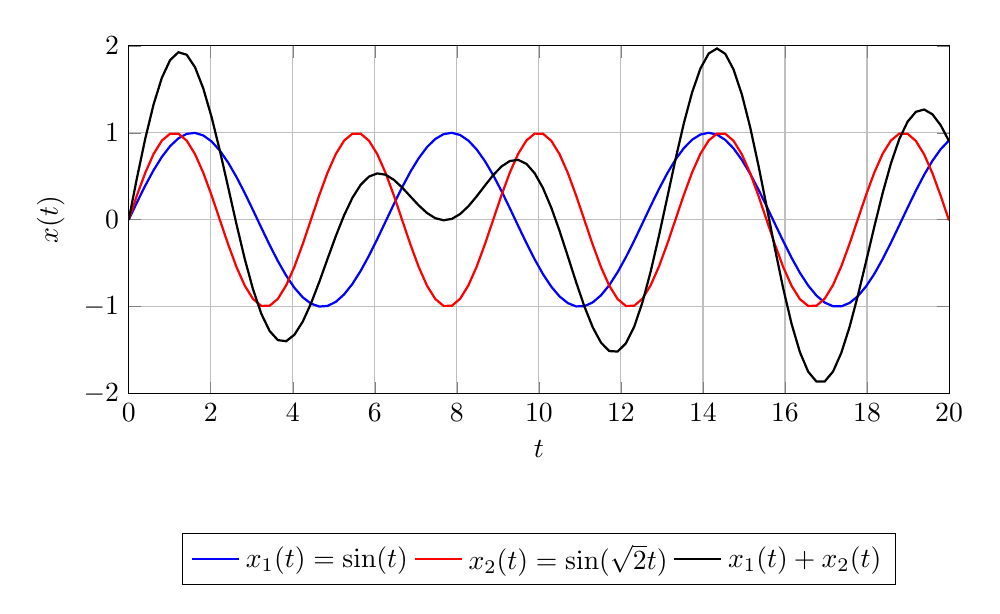
\begin{tikzpicture}
        \begin{axis}[
            width=12cm, height=6cm,
            xlabel={$t$}, ylabel={$x(t)$},
            grid=both,
            legend style={at={(0.5,-0.4)}, anchor=north, legend columns=3},
            xmin=0, xmax=20,
            ymin=-2, ymax=2,
            domain=0:20,
            samples=100
        ]
        \addplot[blue, thick] {sin(deg(x))};         
        \addlegendentry{$x_1(t) = \sin(t)$};
    
        \addplot[red, thick] {sin(sqrt(2) * deg(x))};
        \addlegendentry{$x_2(t) = \sin(\sqrt{2} t)$};
    
        \addplot[thick, black] {sin(deg(x)) + sin(deg(sqrt(2) * x))};
        \addlegendentry{$x_1(t) + x_2(t)$};
        \end{axis}
    \end{tikzpicture}
    \caption{Periodic Signals Sum}
\end{figure}

\section{Unit Step Signal}
The unit step signal, also known as the Heaviside step function, is
0 for values less than 0 and 1 otherwise.

\subsection{Discrete-Time Unit Step Signal}
The discrete-time unit step signal is defined as:
\[
    u[n] =
    \begin{cases}
        1 & n \geq 0, \\
        0 & n < 0.
    \end{cases}
\]
Or alternatively,
\begin{equation}
    u[n] = \sum_{i = -\infty}^{n} \delta[i]
\end{equation}
In either definition,
\[
    u[n] = 1 \text{ for } n \geq 0, \text{ and } u[n] = 0 \text{ for } n < 0.
\]

Figure \ref{fig:dt unit} is the plot for the discrete-time unit step signal.
\begin{figure}[h!]
    \centering
    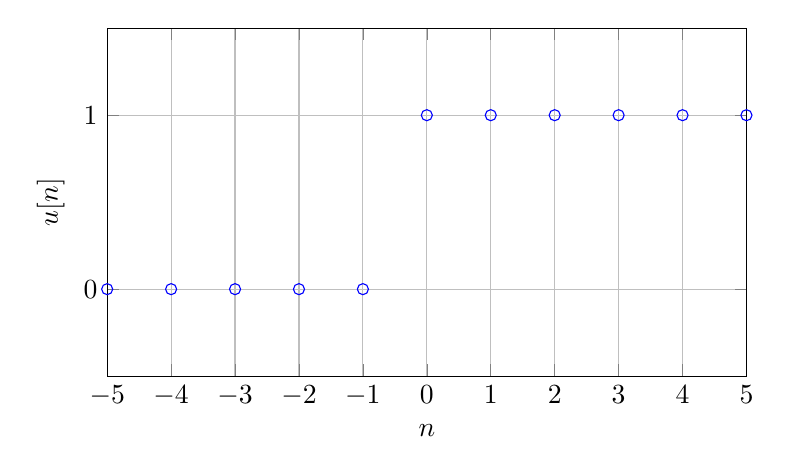
\begin{tikzpicture}
        \begin{axis}[
                xlabel={$n$},
                ylabel={$u[n]$},
                grid=major,
                ytick={0,1},
                xtick={-5,-4,...,5},
                ymin=-0.5, ymax=1.5,
                xmin=-5, xmax=5,
                width=0.8\textwidth,
                height=6cm,
                samples=100,
                domain=-5:5
            ]
            \addplot+[only marks, mark=o] coordinates {
                    (-5,0) (-4,0) (-3,0) (-2,0) (-1,0)
                    (0,1) (1,1) (2,1) (3,1) (4,1) (5,1)
                };
        \end{axis}
    \end{tikzpicture}
    \caption{Discrete-Time Unit Step Signal}
    \label{fig:dt unit}
\end{figure}

A useful property for signal sampling is that, if we
just want to consider a section of the signal between
$0$ and $n_0$, we can just multiply $x[n]$ by $u[n] - u[n - n_0]$.

\subsection{Continuous-Time Unit Step Signal}
The continuous-time unit step signal is defined as:
\[
    u(t) =
    \begin{cases}
        1 & t \geq 0, \\
        0 & t < 0.
    \end{cases}
\]
Or alternatively,
\begin{equation}
    u(t) = \int_{-\infty}^{t} \delta(\tau) d \tau
\end{equation}
We can also make the substitution $\sigma = t - \tau$, which gives
\begin{equation}
    u(t) = \int_0^{\infty} \delta(t - \sigma) d\sigma
\end{equation}

Figure \ref{fig:ct unit} is the plot for the continuous-time unit step signal:

\begin{figure}[h!]
    \centering
    \begin{tikzpicture}
        \begin{axis}[
                xlabel={$t$},
                ylabel={$u(t)$},
                grid=major,
                ytick={0,1},
                xmin=-5, xmax=5,
                ymin=-0.5, ymax=1.5,
                width=0.8\textwidth,
                height=6cm,
                samples=100,
                domain=-5:5
            ]
            \addplot[domain=-5:0, samples=100, thick] {0};
            \addplot[domain=0:5, samples=100, thick] {1};
            \addplot[mark=*, mark size=2pt] coordinates {(0,1)};
        \end{axis}
    \end{tikzpicture}
    \caption{Continuous-Time Unit Step Signal}
    \label{fig:ct unit}
\end{figure}

\subsection{Discrete-Time Delta Function}
The discrete-time delta function, known as the Kronecker delta function, is defined as:
\[
    \delta[n] =
    \begin{cases}
        1 & n = 0,    \\
        0 & n \neq 0.
    \end{cases}
\]

Figure \ref{fig:dt delta} is the plot for the discrete-time delta function:

\begin{figure}[h!]
    \centering
    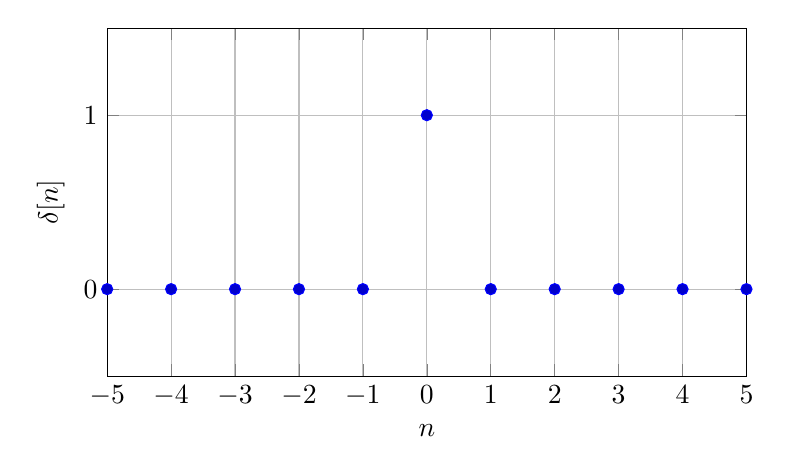
\begin{tikzpicture}
        \begin{axis}[
                xlabel={$n$},
                ylabel={$\delta[n]$},
                grid=major,
                ytick={0,1},
                xtick={-5,-4,...,5},
                ymin=-0.5, ymax=1.5,
                xmin=-5, xmax=5,
                width=0.8\textwidth,
                height=6cm,
                samples=100,
                domain=-5:5
            ]
            \addplot+[only marks, mark=*] coordinates {
                    (-5,0) (-4,0) (-3,0) (-2,0) (-1,0)
                    (0,1) (1,0) (2,0) (3,0) (4,0) (5,0)
                };
        \end{axis}
    \end{tikzpicture}
    \caption{Discrete-Time Delta Function}
    \label{fig:dt delta}
\end{figure}

A useful property of the delta function in DT is that, since
it is just equal to one when its argument is 0, then
\begin{eqnarray}
    x[n] = \sum_{k=-\infty}^{\infty} x[k]\delta [n-k]
\end{eqnarray}

\subsection{Continuous-Time Delta Function}
The continuous-time delta function, known as the Dirac delta
function or unit impulse, is defined as:
\[
    \delta(t) = \begin{cases}
        \infty & t = 0,    \\
        0      & t \neq 0,
    \end{cases}
\]
with the property that:
\[
    \int_{-\infty}^{\infty} \delta(t) dt = 1.
\]

An alternative definition for $\delta(t)$ is
\begin{equation}
    \delta(t) = \frac{d}{dt} u(t)
\end{equation}

Figure \ref{fig:ct delta} is the plot for the continuous-time delta function.
The height of the arrow indicates not the value of the function but its area,
since the value is technically undefined.
\begin{figure}[h!]
    \centering
    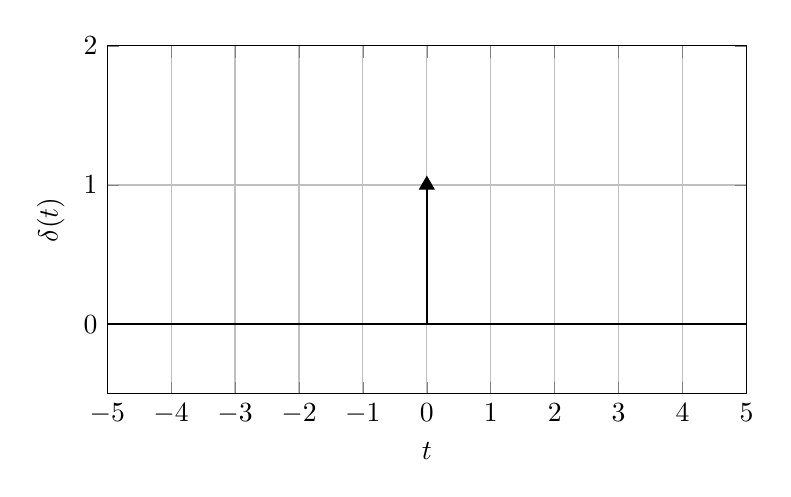
\begin{tikzpicture}
        \begin{axis}[
                xlabel={$t$},
                ylabel={$\delta(t)$},
                grid=major,
                xtick={-5,-4,-3,-2,-1,0,1,2,3,4,5},
                ymin=-0.5, ymax=2,
                xmin=-5, xmax=5,
                width=0.8\textwidth,
                height=6cm,
                samples=100
            ]
            \addplot[thick, domain=-5:5, samples=2] {0};
            \addplot[only marks, mark=triangle*, mark size=3pt] coordinates {(0,1)};
            \addplot[thick] coordinates {(0,0) (0,1)};
        \end{axis}
    \end{tikzpicture}
    \caption{Continuous-Time Delta Function}
    \label{fig:ct delta}
\end{figure}

The \emph{sampling property} is the property that
\begin{equation}
    x(t) \delta(t - \sigma) = x(\sigma) \delta(t - \sigma).
\end{equation}

We can decompose $x(t)$
\begin{align}
    x(t) & = x(t) \times 1                                                  \\
         & = x(t) \int_{-\infty}^{\infty} \delta(t - \sigma) d \sigma       \\
         & = \int_{-\infty}^{\infty} x(t) \delta(t - \sigma) d \sigma       \\
         & = \int_{-\infty}^{\infty} x(\sigma) \delta(t - \sigma) d \sigma.
\end{align}
In DT, this becomes
\begin{equation}
    x[n] = \sum_{k=-\infty}^{\infty} x[k] \delta[n - k]
\end{equation}
\section{Complex Exponential}
A CT complex exponential signal is of the form 
$x(t) = Ce^{\alpha t}$, where $C$ and $\alpha$ 
are in general complex. Alternatively, 
\begin{equation}
    x(t) = |C| e^{\sigma t} e^{j(\omega t + \phi)}
\end{equation}
where $\phi$ is the angle between the real axis and 
$C$ when plotted on the complex plane and $\alpha = \sigma + j\omega$. 

The $\sigma$ term determines whether the signal has exponential 
growth, decay, or neither. If $\sigma = 0$ then we are left 
with the periodic complex exponential $e^{j(\omega t + \phi)}$ 
with period $\frac{2\pi}{\omega}$. 

$\omega$ is called the fundemental frequency, 
$\phi$ is called the phase. 

The signal $x(t) = |C|e^{\sigma t}e^{j(\omega t + \phi)}$
forms a family of signals called harmonically 
related complex exponentials (HRCEs), each of the 
form 
\begin{equation}
    x_k(t) = e^{jk\omega_0 t}, k \in \mathbb{Z}.
\end{equation}
These signals will serve as our building 
blocks when we construct Fourier series 
of complex exponential signals later on. 

Let's now look at the discrete time 
complex exponential,
\begin{equation}
    x[n] = C \alpha^n.
\end{equation}
In general, $C$ and $\alpha$ can be complex. 
This can be rewritten 
\begin{eqnarray}
    x[n] = |C|e^{\sigma n} e^{j(\omega n + \phi)}. 
\end{eqnarray}
Where the continuous and discrete begin 
to diverge is when we consider the 
$e^{j(\omega n + \phi)}$ term. This 
term is not always periodic, unlike 
the case of continuous time. For 
the CT case, the fundemental 
frequency is $\omega$ and larger 
values of $\omega$ produce 
higher rates of oscillation. 

Now say we want to compute the 
fundemental period of $x[n] = \cos(3\pi n)$. 
In the continuous case it's easy, $\frac{2}{3}$.
In the discrete case, we need to 
find the least common multiple 
of the fundemental period 
of the CT signal (in this case, 
$\frac{2}{3}$) and the sampling 
period. This is why the 
discrete case may not be periodic.
Imagine the sampling period is 1
and the fundemental period of the 
CT signal is $2 \pi$. Then the 
least common multiple does not 
exist. 

Let's do an example problem. 
Consider the signal 
\begin{eqnarray}
    x(t) = e^{j2t} + e^{j5t}.
\end{eqnarray}
We can rewrite this, using 
the identity 
\begin{equation}
    \cos(\omega t) = \frac{e^{-j \omega t}+ e^{j\omega t}}{2}
\end{equation}
to the expression 
\begin{align}
    e^{j 3.5 t} (e^{j1.5t} + e^{-j 1.5 t}) \\
    &= 2 e^{j 3.5 t}\cos(1.5t) \\
    |x(t)| &= 2|\cos(1.5 t)|
\end{align}

\begin{align}
    x[n] &= C\alpha^n \\
    &= Ce^{\beta n}
\end{align}
is the general form of a discrete complex exponential and 
$\beta$ is in general complex. If $\alpha$ is real and less 
than 0, then $\beta$ must be complex. 

\section{System Connections}

Often we analyze a complex system as a set of subsystems
connected to one another. These connections can take
many forms, but some of the more common ones are in series,
parallel, and feedback.

\subsection{Series}

\begin{equation}
    y(t) = S_2(S_1(x(t)))
\end{equation}

\begin{figure}[ht]
    \centering
    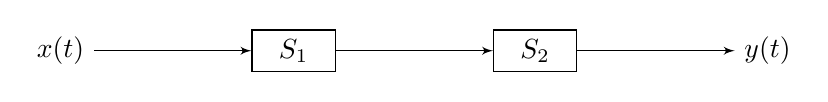
\begin{tikzpicture}[node distance=2cm, auto, >=latex']
        \node (input) {$x(t)$};
        \node[block, right= of input] (s1) {$S_1$};
        \node[block, right= of s1] (s2) {$S_2$};
        \node[right= of s2] (output) {$y(t)$};

        \draw[->] (input) -- (s1);
        \draw[->] (s1) -- (s2);
        \draw[->] (s2) -- (output);
    \end{tikzpicture}
    \caption{Series connection block diagram.}
\end{figure}

\subsection{Parallel}

\begin{equation}
    y(t) = S_1(x(t)) + S_2(x(t))
\end{equation}

\begin{figure}[ht]
    \centering
    \begin{tikzpicture}[node distance=2cm, auto, >=latex']
        \node (input) {$x(t)$};
        \coordinate[right= of input] (split);
        \node[block, above right= of split] (s1) {$S_1$};
        \node[block, below right= of split] (s2) {$S_2$};
        \node[sum, right=4cm of split] (sum) {+};

        \draw[->] (input) -- (split);
        \draw[->] (split) |- (s1);
        \draw[->] (split) |- (s2);
        \draw[->] (s1) -| (sum);
        \draw[->] (s2) -| (sum);
        \draw[->] (sum) -- node {$y(t)$} ++(1,0);
    \end{tikzpicture}
    \caption{Parallel connection block diagram.}
\end{figure}

\subsection{Feedback}

\begin{equation}
    y(t) = S_1\left( x(t) - S_2(y(t)) \right)
\end{equation}

\begin{figure}[ht]
    \centering
    \begin{tikzpicture}[node distance=2cm, auto, >=latex']
        \node (input) {$x(t)$};
        \node[sum, right= of input] (sum) {$\Sigma$};
        \node[block, right= of sum] (s1) {$S_1$};
        \node[right= of s1] (output) {$y(t)$};
        \node[block, below= of s1] (s2) {$S_2$};

        \draw[->] (input) -- node[above left] {+} (sum);
        \draw[->] (sum) -- (s1);
        \draw[->] (s1) -- (output);
        \draw[->] (output) |- (s2);
        \draw[->] (s2) -| node[pos=0.95, left] {-} (sum);
    \end{tikzpicture}
    \caption{Feedback connection block diagram.}
\end{figure}
\section{System Properties}

\subsection{Memoryless}
A \emph{mempryless} system output is dependent
only on the input at time $t$, and not previous states.

\subsection{Invertable}
A system is \emph{invertable} is distinct
inputs lead to distinct outputs. A system is not
invertable if there exists any $x(t) \new x_2(t)$ such
that $y_1(t) = y_2(t)$.

\subsection{Linear}



\section{Reference}
\begin{itemize}
    \item $E = mc^2$
\end{itemize}

\end{document}